\section{Modélisation}

	L'analyse préalable nous permet à présent d'avoir une vision plus précise des fonctionnalités de notre programme en vue de réaliser son diagramme de classe. Pour simplifier la modélisation et permettre une plus grande modularité de nos classes nous avons voulu utiliser un maximum des patrons de conceptions. 

	\subsection{patron de Conception}

		\subsubsection{Monteur : création d'une partie}

		\textbf{Bedbihan} permet aux joueurs de jouer différentes type de parties. Ainsi il existe différentes manières de construire une partie en fonction du type désiré. Néanmoins ces créations passent par des étapes similaires : création de la carte, créations des unités, etc. C'est pourquoi sur  la création de la partie est assurée par le patron de conception \textbf{Monteur}. Ce patron de conception nous permet de séparer la conception de l'objet \emph{Game} de sa représentation. Ainsi cette étapes gagne en flexibilité. 

		\begin{figure}[h]
		\begin{center}
			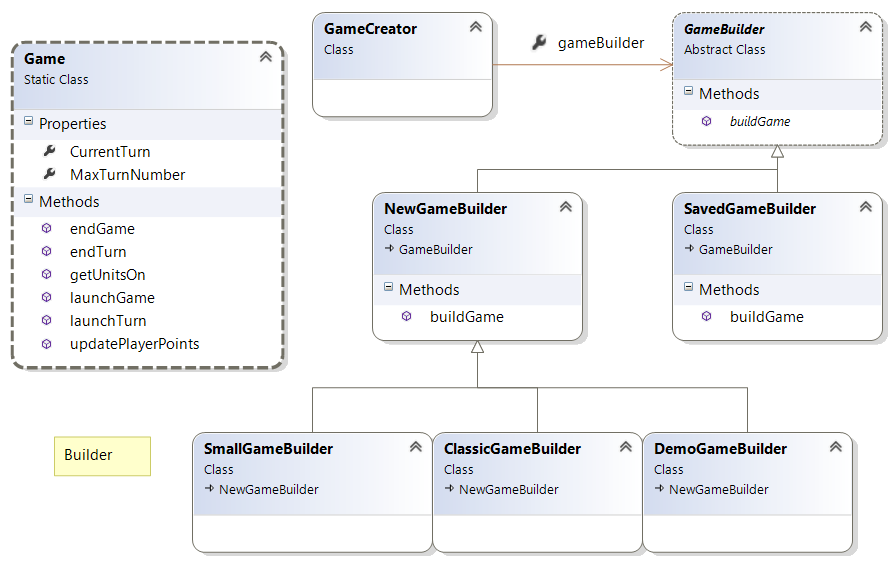
\includegraphics[width=0.5\textwidth]{figure/builder.png}
		\end{center}
		\caption{Création de la partie : patron de conception Monteur}
		\label{fig:builder}
	\end{figure}

		\subsubsection{Fabrique : création de différents peuples}

		
		La création des peuples est assurée par le patron de conception de création \textbf{Fabrique}. Ce patron de conception nous permettra de créer l'armée adéquate en fonction du peuple choisie par le joueur au lancement de la partie. 
		\subsubsection{Poids-Mouche : ne sert a rien}

		\subsubsection{Stratégie : création des différents type de carte}


%		\begin{figure}[h]
%			\begin{center}
%				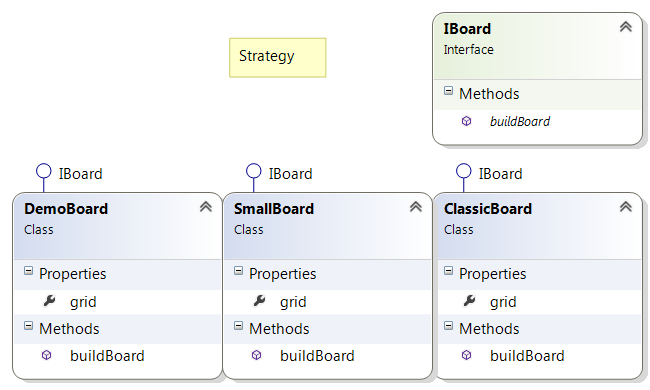
\includegraphics[width=0.5\textwidth]{figure/strategy.png}
%			\end{center}
%			\caption{Implémentations du plateau de jeu : patron de conception strategie}
%			\label{fig:strategy}
%		\end{figure}

		La création des cartes, de tailles fixes mais dont la composition des dalles est implémentée de maniére aléatoire, repose sur le patron de conception \emph{stratégie}. Ce patron de conception nous permet de choisir de manière précise l'algorithme de création de carte désiré. De plus, il permet une grande flexibilité pour définir de nouveaux types de cartes.



	\subsection{Diagramme de classe}


	\begin{figure}
		\begin{center}
			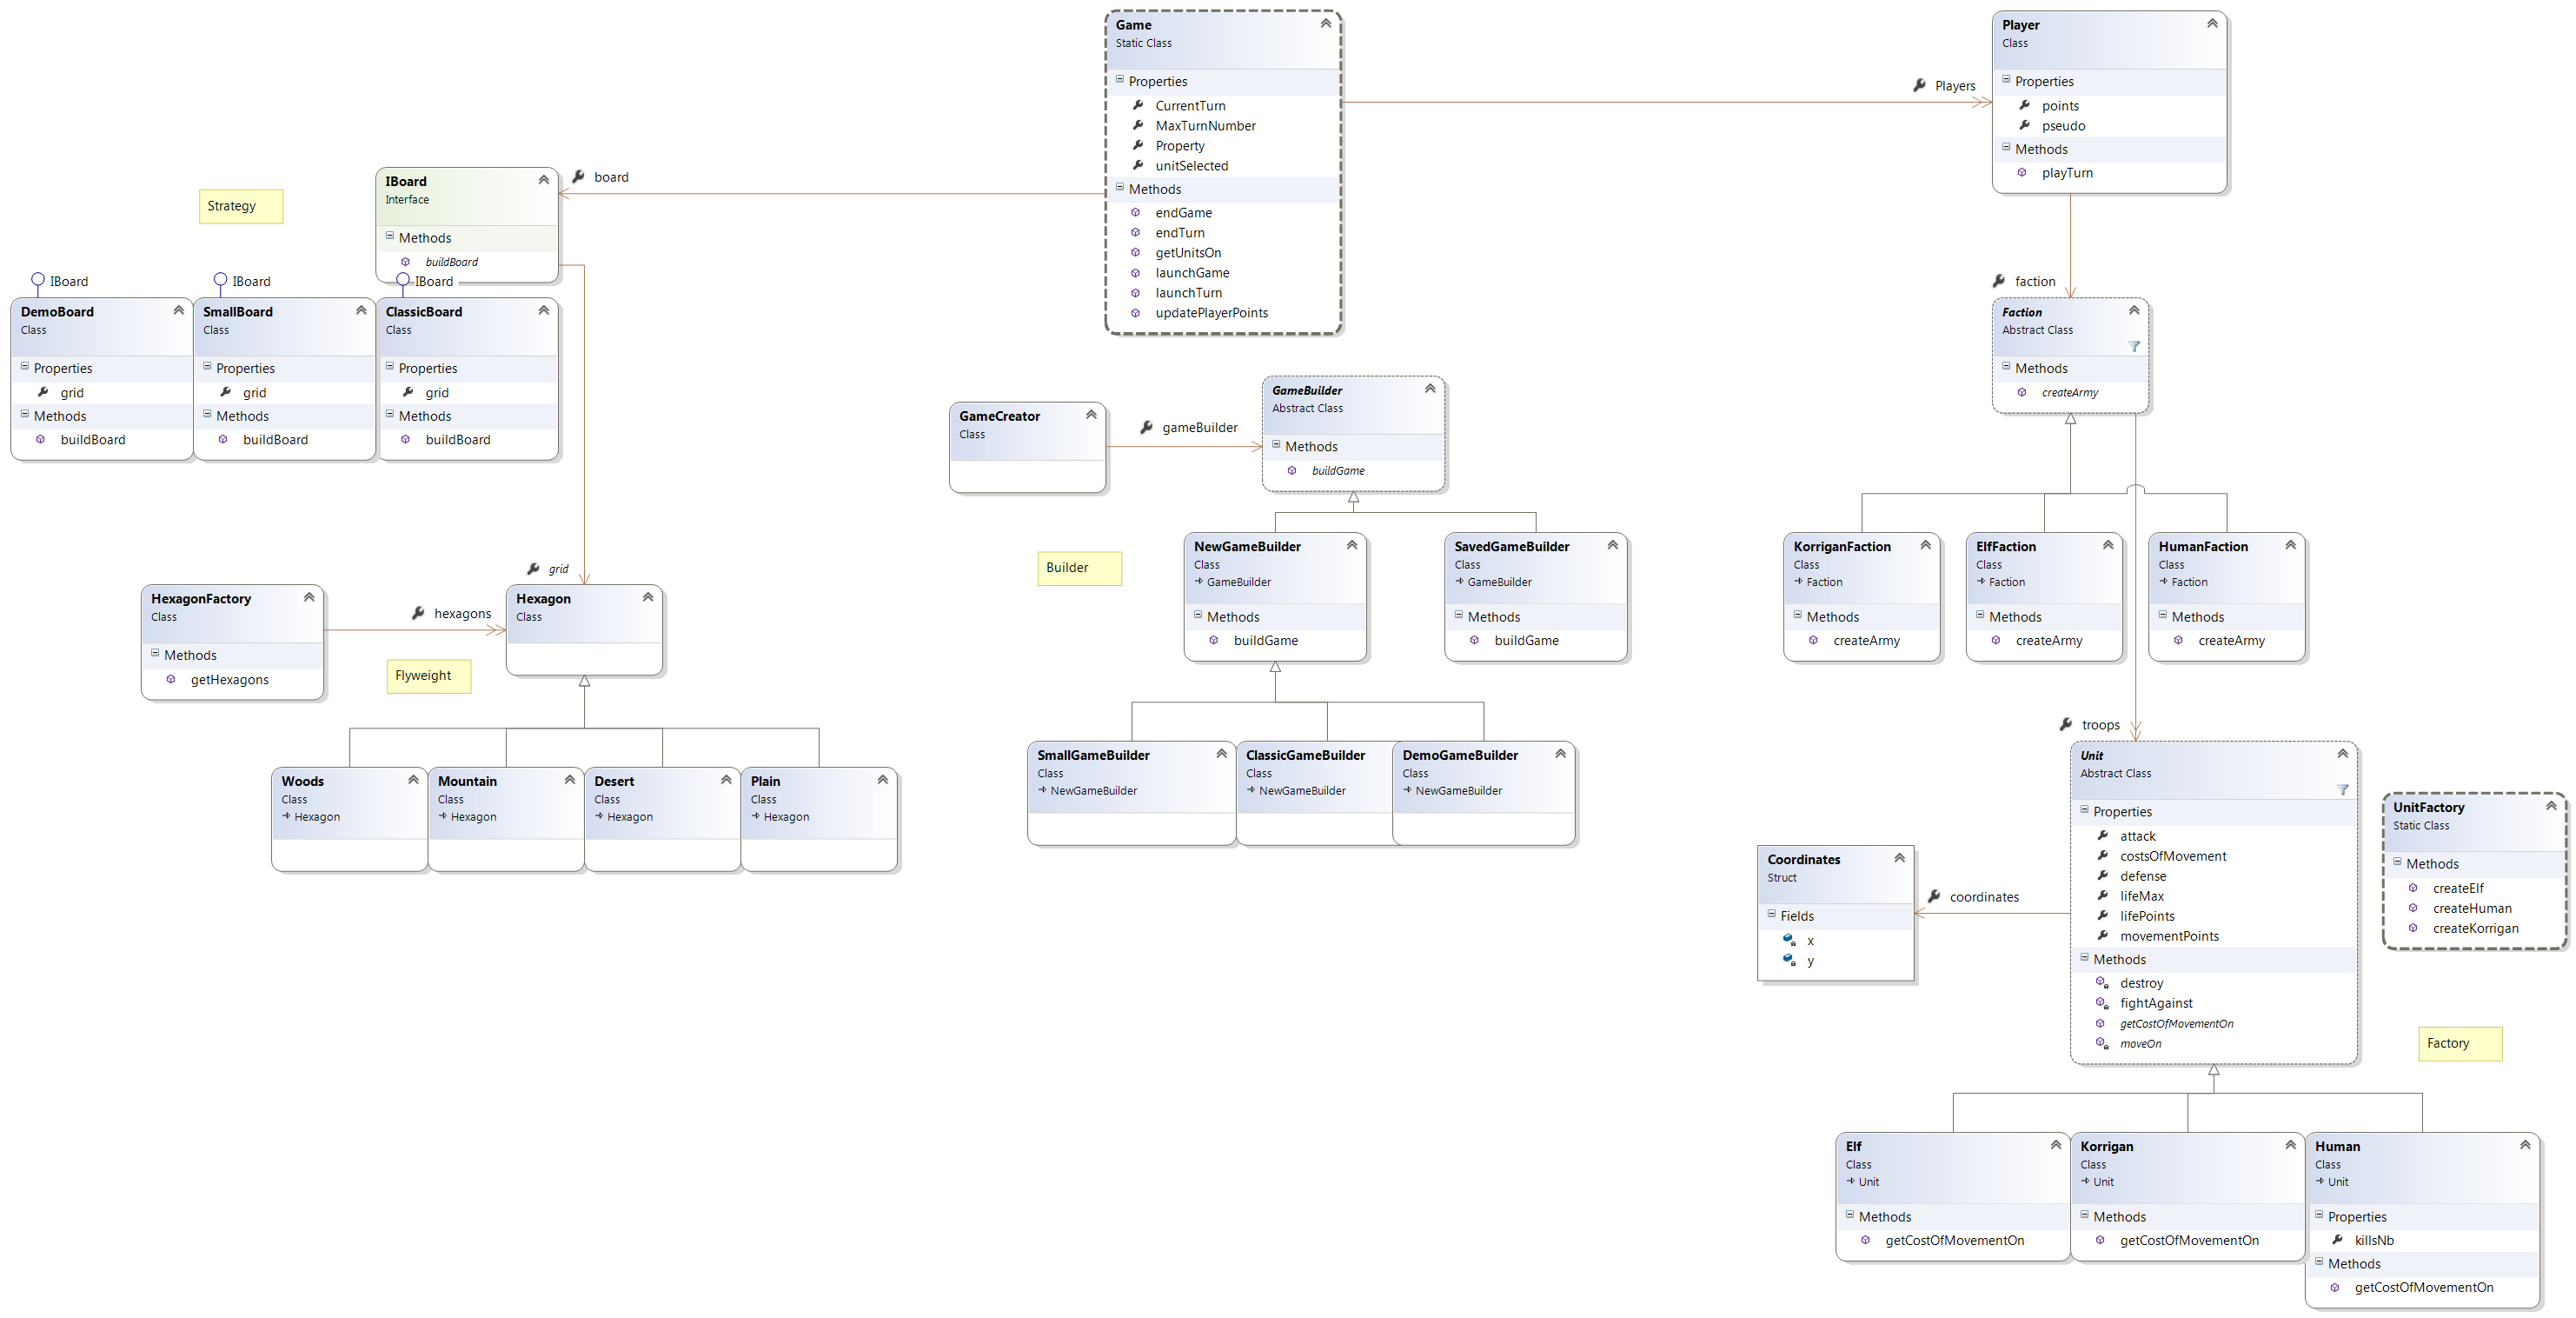
\includegraphics[width=0.5\textwidth]{figure/entire_class_diagram}
		\end{center}
		\caption{Diagrame de classe}
		\label{fig:planif}
	\end{figure}




